\documentclass[../main.tex]{subfiles}

\begin{document}
\begin{questions}

\question Two co-planar dipoles are oriented as shown in the figure. Find equilibrium value of $\theta^\prime$ if $\theta$ is fixed.
\begin{center}
	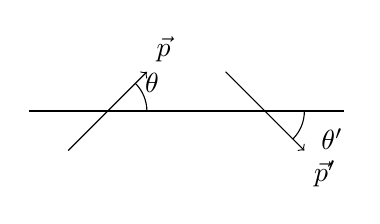
\begin{tikzpicture}
		\draw[thick] (0,0) -- (4,0);
		\draw[->] (0.5,-0.5) -- (1.5,0.5) node[above right]{$\vec{p}$};
		\draw (1.5,0) arc (0:45:0.5) node[right]{$\theta$};

		\draw[<-] (3.5,-0.5) node[below right]{$\vec{p}^\prime$} -- (2.5,0.5);
		\draw (3.5,0) arc (0:-45:0.5) node[xshift=0.5cm]{$\theta^\prime$};
	\end{tikzpicture}
\end{center}
\begin{solution}
	In equilibrium, the energy of the system will be minimized (or maximized).

	The positions of $\vec{p}$ and $\vec{p}^\prime$ are fixed, so the only degree of freedom the energy depends on is the orientation of $\vec{p}^\prime$. The energy of $\vec{p}^\prime$ in the field of $\vec{p}$ will be minimized (or maximized) when $\vec{p}^\prime$ is along (or opposite to) $\vec{E}_{\vec{p}}$.

	We can easily find the direction of $\vec{E}_{\vec{p}}$ at $\vec{p}^\prime$. Let the distance between the dipoles be $\vec{r}$, and let the axis joining their centres be the $x$ axis, and the dipoles be oriented in the $xy$ plane
	\begin{align}
		\vec{E}_{\vec{p}} &= \frac{1}{4\pi\epsilon_0}\frac{2|\vec{p}|\cos\theta}{r^2}\,\ihat - \frac{1}{4\pi\epsilon_0}\frac{|\vec{p}|\sin\theta}{r^3}\,\jhat\\
		\implies \tan(\theta^\prime) &= \frac{-\vec{E}_{\vec{p}}\cdot \jhat}{\vec{E}_{\vec{p}}\cdot \ihat}\\
		&= \frac{\sin\theta}{2\cos\theta}\\
		&= \frac{\tan(\theta)}{2}\\
		\implies \theta^\prime &= \tan^{-1}\left(\frac{\tan(\theta)}{2}\right)
	\end{align}
	Thus the dipole will align itself along (or opposite to) $\theta^\prime$
\end{solution}

\question Let $I$ be the current carried by a wire bent into a planar loop. Place the origin of coordinates at an observation point $\vec{P}$ in the plane of the loop.
\label{q:mag}
\begin{parts}
	\part Show that the magnitude of the magnetic field at the point $\vec{P}$ is
	\label{part:mag}
	\begin{equation*}
		|\vec{B}(\vec{P})| = \frac{\mu_0I}{4\pi}\int_0^{2\pi}\frac{d\phi}{r(\phi)}
	\end{equation*}
	where $r(\phi)$ is the distance from the origin of coordinates at $\vec{P}$ to the point on the loop located at an angle $\phi$ from the positive $x$ axis.
	\begin{solution}
		To obtain the limits of the integral mentioned in the question, we have to assume the point lies \textit{inside} the loop.

		\begin{center}
			\begin{tikzpicture}
				\draw[->] (0,0) -- (0,4) node[above]{$y$};
				\draw[->] (0,0) -- (4,0) node[right]{$x$};
			
				\node at (0,0)[left]{$\vec{P}$};

				\draw (0.8,0.4) circle (2.5);

				\def\th{atan((0.4+2.5*sin(55))/(0.8+2.5*cos(55)))};

				\draw (0,0) -- ({0.8+2.5*cos(55) - 1.5*cos(\th)},{0.4+2.5*sin(55) - 1.5*sin(\th)});

				\draw[<-] ({0.8+2.5*cos(55) - 1.5*cos(\th)},{0.4+2.5*sin(55) - 1.5*sin(\th)}) node[above left]{$\vec{r}$} -- +({1.5*cos(\th)},{1.5*sin(\th)});


				% \draw[dotted] ({0.8+2.5*cos(55)},{0.4+2.5*sin(55)}) -- +({0.5*cos(\th)},{0.5*sin(\th)});

				% \draw ({0.8+2.5*cos(55) + 0.25*cos(\th)},{0.4+2.5*sin(55) + 0.25*sin(\th)}) arc ({\th}:{180-35}:0.25) node[above]{$\theta$};

				\draw (0.25,0) arc (0:{\th}:0.25) node[right]{$\phi$};

				% \draw[dotted] ({0.8+2.5*cos(55)},{0.4+2.5*sin(55)}) -- ({0.8+2.5*cos(55)+(0.4+2.5*sin(55))/(sin(35))},0);

				% \draw ({1.05+2.5*cos(55)+(0.4+2.5*sin(55))/(sin(35))},0) arc (0:{180-35}:0.25) node[above right]{$\alpha$};

				\draw[thick,Latex-] ({0.8+2.5*cos(55)-0.6*cos(35)},{0.4+2.5*sin(55)+0.6*sin(35)}) -- +({1.2*cos(35)},{-1.2*sin(35)}) node[yshift=0.5cm]{$I\,d\vec{l}$};
			\end{tikzpicture}
		\end{center}

		\begin{align}
			\vec{B}(\vec{P}) &= \frac{\mu_0I}{4\pi}\oint\frac{d\vec{l}\times\hat{r}}{|\vec{r}|^2}\\
			&= \frac{\mu_0I}{4\pi}\oint\frac{ \left(dr\,\hat{r}+|\vec{r}|\,d\phi\,\hat{\phi}\right)\times\hat{r}}{|\vec{r}|^2}\\
			&= \frac{\mu_0I}{4\pi}\oint \frac{d\phi}{|\vec{r}|}\,d\khat\\
			\implies |\vec{B}(\vec{P})| &= \frac{\mu_0I}{4\pi}\int_{\phi=0}^{2\pi} \frac{d\phi}{|\vec{r}|}
		\end{align}
	\end{solution}

	\part Show that the magnetic field at the center of a current-carrying wire	bent into an ellipse with major and minor axes $2a$ and $2b$ is proportional to the integral of the form (with constant $k$),
	\begin{equation*}
		\int_{0}^{\frac{\pi}{2}} d\phi\sqrt{1-k^2\sin^2\phi}
	\end{equation*}
	What are the magnetic fields when $a = b$ and when $a \to \infty$ with $b$ fixed?
	\begin{solution}
		Applying the result obtained in the previous part,
		\begin{align}
			r(\phi) &= \frac{ab}{\sqrt{a^2\sin^2\phi+b^2\cos^2\phi}}\\
			\implies |\vec{B}(\vec{P})| &= \frac{\mu_0I}{4\pi} \int_{\phi=0}^{2\pi} \frac{\sqrt{a^2\sin^2\phi+b^2\cos^2\phi}}{ab}\,d\phi\\
			&= \boxed{\frac{\mu_0I}{\pi a}\int_{\phi=0}^{\frac{\pi}{2}}\sqrt{1-\left(1-\frac{a^2}{b^2}\sin^2\phi\right)}\,d\phi}
		\end{align}
		When $a=b$
		\begin{align}
			|\vec{B}(\vec{P})| &= \frac{\mu_0I}{\pi a}\int_{\phi=0}^{\frac{\pi}{2}} \,d\phi = \frac{\mu_0I}{2a}
		\end{align}
		When $a\to\infty$
		\begin{align}
			|\vec{B}(\vec{P})| &= \frac{\mu_0I}{\pi b}\int_{\phi=0}^{\frac{\pi}{2}} \sin\phi\,d\phi = \frac{\mu_0I}{\pi b}
		\end{align}
	\end{solution}

	\part An infinitesimally thin wire is wound in the form of a planar coil which can be modeled using an effective surface current density $\vec{K}=K\,\hat{\phi}$. Find the magnetic field at a point $\vec{P}$ on the symmetry axis of the coil. Express your answer in terms of the angle $\alpha$ subtended by the coil at P.

	\begin{solution}
		\begin{center}
			\tdplotsetmaincoords{60}{105}
			\begin{tikzpicture}[tdplot_main_coords]
				\draw[thick,->] (0,0,0) -- (4,0,0) node[anchor=north]{$x$};
				\draw[thick,->] (0,0,0) -- (0,4,0) node[anchor=west]{$y$};
				\draw[thick,->] (0,0,0) -- (0,0,4) node[anchor=south]{$z$};
				

				\begin{scope}[canvas is xy plane at z=0]
					\draw (0,0) circle (2.5);

					\draw (0.5,0) arc (0:70:0.5) node[below]{$\phi$};
					\draw[dotted] (0,0) -- ({2*cos(70)},{2*sin(70)});

					\draw[thick,->]  ({2*cos(70)+0.3*cos(20)},{2*sin(70)-0.3*sin(20)}) -- +({-0.6*cos(20)},{0.6*sin(20)});
				\end{scope}

				\begin{scope}[canvas is plane={O(0,0,3)x(0,0,2)y({cos(70)},{sin(70)},3)}]
					\draw (0.5,0) node[below right]{$\lambda$} arc (0:{atan(2/3)}:0.5);
				\end{scope}

				\draw (0,0,3) node[left]{$\vec{r}$} -- ({2*cos(70)},{2*sin(70)},0) node[yshift=-0.2cm, xshift=-0.6cm]{$\vec{r}^\prime$};
			\end{tikzpicture}

			\begin{align}
				\vec{\rcurs} &= \vec{r} - \vec{r}' = z\,\khat - r^\prime\,\hat{r}\\
				\vec{B}(\vec{r}) &= \frac{\mu_0}{4\pi}\iint \frac{\vec{K}(\vec{r^\prime})\times \hat{\rcurs}}{\rcurs^2}\,dS\\
				&= \frac{\mu_0K}{4\pi} \iint \frac{\hat{\phi}\times\vec{\rcurs}}{(z^2+r'^2)^{\frac{3}{2}}}\,dS\\
				&= \frac{\mu_0K}{4\pi} \iint \frac{(-\sin\phi\,\ihat+\cos\phi\,\jhat)\times(z\,\khat - r^\prime \cos\phi\,\ihat - r^\prime \sin\phi\,\jhat)}{(z^2+r'^2)^{\frac{3}{2}}}\,dS
			\end{align}
			\begin{align}
				= \frac{\mu_0K}{4\pi}\left(\int_{r'=0}^{R}\cancelto{0}{\int_{\phi=0}^{2\pi} \frac{z\cos\phi}{(z^2+r'^2)^\frac{3}{2}}r'\,d\phi\,dr'}\,\ihat + \int_{r'=0}^{R}\cancelto{0}{\int_{\phi=0}^{2\pi} \frac{z\sin\phi}{(z^2+r'^2)^\frac{3}{2}}r'\,d\phi\,dr'}\,\jhat\right.\nonumber
			\end{align}
			\begin{align}
				&+\left. \int_{r'=0}^{R}\int_{\phi=0}^{2\pi} \frac{r'^2}{(z^2+r'^2)^\frac{3}{2}}\,d\phi\,dr'\,\khat \right)\\
				&= \frac{\mu_0K}{2}\int_{r'=0}^{R} \frac{r'^2}{(z^2+r'^2)^\frac{3}{2}}\,dr'\,\khat\\
				&= \frac{\mu_0K}{2}\int_{\lambda=0}^{\alpha} \left(\sec\lambda - \cos\lambda\right)\,d\lambda\,\khat\\
				&= \frac{\mu_0K}{2}\left(\ln(\sec\alpha + \tan\alpha)-\sin\alpha\right)
			\end{align}
		\end{center}
	\end{solution}
\end{parts}

\question A circular loop of wire carries a current $I_1$. A long straight wire in the plane of the loop carries a current $I_2$. The loop subtends an angle $2\theta$ at a point on the wire which is nearest to it. Show that the force between the wire and the loop has a magnitude $\mu_0I_1I_2(\sec\theta-1)$

\begin{solution}
	\begin{center}
		\begin{tikzpicture}
			\draw[thick,->] (0,0) -- (4,0) node[right]{$x$};
			\draw[thick,->] (0,0) -- (0,4) node[above]{$y$};

			\draw[->] (2,0) arc (0:45:2) node[right]{$I_1$};
			\draw ({2*cos(45)},{2*sin(45)}) arc (45:360:2);

			\draw (0.6,0) arc (0:45:0.6) node[right]{$\phi$};

			\draw[dashed] (-4,-4) -- (-3,-4);
			\draw[dashed] (3,-4) -- (4,-4); 
			\draw[->] (-3,-4) -- (-1,-4) node[above left]{$I_2$};
			\draw (-1,-4) -- (3,-4);

			\def\th{asin(0.5)};

			\draw[dotted] (0,-4) -- +({sqrt(12)*sin(\th)},{sqrt(12)*cos(\th)});
			\draw[dotted] (0,-4) -- +({-sqrt(12)*sin(\th)},{sqrt(12)*cos(\th)});

			\draw[dashed] (0,-4) -- (0,-2);

			\draw ({0.6*sin(\th)},{-4+0.6*cos(\th)}) arc ({90-\th}:90:0.6) node[above right]{$\theta$};

			\draw[dotted] (0,0) -- ({sqrt(2)},{sqrt(2)});

			\draw[decorate,decoration={brace, raise=5pt, amplitude=5pt, mirror}] (2,-3.8) -- node[right=7pt]{$R\csc\theta$} (2,-0.2);
		\end{tikzpicture}
	\end{center}

	Let us find force on $I_1$ due to field of $I_2$
	\begin{align}
		\vec{B}_{I_2}(\phi) &= \frac{\mu_0I_2}{2\pi(R\sin\phi + R\csc\theta)}\,\khat\\
		\implies \vec{F} &= \oint I_1\,d\vec{l}\times\vec{B}_{I_2}(\phi)\\
		&=  \frac{\mu_0I_1I_2}{2\pi} \int_{\phi=0}^{2\pi} \frac{d\phi}{\sin\phi+\csc\theta}\,\hat{\phi}\times\khat\\
		&= \frac{\mu_0I_1I_2}{2\pi} \int_{\phi=0}^{2\pi} \frac{d\phi}{\sin\phi+\csc\theta}\,(-\sin\phi\,\ihat+\cos\phi\,\jhat)\times\khat\\
		&= \frac{\mu_0I_1I_2}{2\pi} \left(\cancelto{0}{\int_{\phi=0}^{2\pi} \frac{\cos\phi\, d\phi}{\sin\phi+\csc\theta}}\,\ihat\right.\\
		&+ \left.\int_{\phi=0}^{2\pi} \frac{\sin\phi \,d\phi}{\sin\phi+\csc\theta}\,\jhat\right)\\
		&= \frac{\mu_0I_1I_2}{2\pi}\left(2\pi-\csc\theta\int_{\phi=0}^{2\pi}\frac{1}{\sin\phi+\csc\theta}\,d\phi\right)\,\jhat\\
		&= -\mu_0I_1I_2(\sec\theta-1)\,\jhat
	\end{align}
\end{solution}

\question A long cylindrical conductor of radius R carries current through it, with current density $J = kr$. Find the expression for magnetic field B at a distance $r$ $(r < R)$.
\begin{solution}
	Using Ampere's Law,
	\begin{align}
		\iint \vec{J}\cdot d\vec{a} &= \oint B\cdot d\vec{l}
		\intertext{Using symmetry, magnetic field is independent of $\theta$ and using the fact that its divergence is 0, the radial component of B is also 0} 
		\implies \int_0^rkr\cdot 2\pi r dr &= B\cdot 2\pi r\\
		\implies B &= \frac{kr^2}{3}
	\end{align}
\end{solution}

\question Calculate the force between two closed circuits carrying steady currents.
\label{q:mag1}
\begin{solution}
	\begin{center}
		\begin{tikzpicture}
			\draw[rotate=25] (0,0) ellipse (3 and 2.5);

			\draw[->,rotate=25] (0,2.5) -- (-0.01,2.5) node[above left]{$I_2$};

			\draw (7,0) ellipse (2.5 and 3);
			\draw[<-] (7,-3) -- (6.99,-3) node[below]{$I_1$};

			\draw[thick,->] (0,0) -- (2,0) node[right]{$x$};
			\draw[thick,->] (0,0) -- (0,4) node[above]{$y$};

			\draw[dotted] ({2.5*sin(25)}, {-2.5*cos(25)}) -- node[right=12pt, yshift=3pt]{$\vec{\rcurs}$} (7,3);

			\draw[->] (0,0) -- ({2.5*sin(25)}, {-2.5*cos(25)}) node[above left=3pt]{$\vec{r}_2$};
			\draw[->] (0,0) -- (7,3) node[above left]{$\vec{r}_1$};
		\end{tikzpicture}
	\end{center}

	\begin{align}
		\vec{B}(\vec{r}_1) &= \frac{\mu_0I_2}{4\pi}\oint_2 \frac{d\vec{l}_2\times\vec{\rcurs}}{|\vec{\rcurs}|^3}\\
		&= \frac{\mu_0I_2}{4\pi}\oint_2 \frac{d\vec{l}_2\times(\vec{r}_1-\vec{r}_2)}{|\vec{r}_1-\vec{r}_2|^3}\\
		\implies \vec{F}_{12} &= I_1 \oint_1 d\vec{l}_1\times\vec{B}(\vec{r}_1)\\
		&= \frac{\mu_0I_1I_2}{4\pi} \oint_1 \oint_2 \frac{d\vec{l}_1\times(d\vec{l}_2\times(\vec{r}_1-\vec{r_2}))}{|(\vec{r}_1-\vec{r_2})^3|}\\
		&= \frac{\mu_0I_1I_2}{4\pi} \left(\oint_2 d\vec{l}_2\oint_1 \frac{d\vec{l}_1\cdot(\vec{r}_1-\vec{r_2})}{|(\vec{r}_1-\vec{r_2})^3|}\right.\nonumber\\
		&- \left.\oint_2\oint_1 (\vec{r}_1-\vec{r_2})\frac{d\vec{l}_1\cdot d\vec{l}_2}{|\vec{r}_1-\vec{r_2}|^3}\right) & \text{$\because$ BAC-CAB rule}
	\end{align}
	\begin{align}
		&= -\frac{\mu_0I_1I_2}{4\pi} \left(\oint_2 d\vec{l}_2\cancelto{0}{\oint_1 \nabla\left(\frac{1}{|\vec{r}_1-\vec{r}_2|}\right)\cdot d\vec{l}_1} \right.\nonumber\\
		&- \left.\oint_2\oint_1 (\vec{r}_1-\vec{r_2})\frac{d\vec{l}_1\cdot d\vec{l}_2}{|\vec{r}_1-\vec{r}_2|^3}\right)\\
		&= \frac{\mu_0I_1I_2}{4\pi} \oiint_{1,2} \frac{\vec{r}_2-\vec{r}_1}{|\vec{r}_1-\vec{r}_2|^3}\,d\vec{l}_1\cdot d\vec{l}_2
	\end{align}
\end{solution}

\question Using Biot and Savart law, find $\vec{B}(\vec{r})$ in the plane of the wire at a distance $d$ from the bend along the axis of symmetry.

\begin{solution}

	\begin{center}
		\begin{tikzpicture}
			\draw[dotted] (0,0) -- (4,0);
	
			\node at (1,0){\textbullet};
	
			\draw[decorate, decoration={brace, raise=5pt, amplitude=5pt, mirror}] (1,0) -- node[below=10pt]{$d$} (3,0);
	
			\begin{scope}[very thick,decoration={
				markings,
				mark=at position 0.5 with {\arrow{>}}}
				] 
				\draw[very thick, postaction={decorate}] (5,5) -- node[right]{$I$} (3,0);
				\draw[very thick, postaction={decorate}] (3,0) -- node[right]{$I$} (5,-5);
			\end{scope}
	
			\begin{scope}
				\path[clip] (5,5) -- (3,0) -- (5,-5) -- cycle;
	
				\draw (3,0) node[above right=9pt]{$\alpha$} circle (0.6);
			\end{scope}

			\begin{scope}
				\path[clip] (5,5) -- (3,0) -- (0,0) -- cycle;

				\draw[dashed] (1,0) -- (4,2);

				\draw[decorate,decoration={brace, raise=5pt,amplitude=5pt}] (1,0) -- node[midway, above=10pt, sloped]{$\frac{d\sin\alpha}{\sin(\alpha-\phi)}$} (4,2);
			\end{scope}

			\begin{scope}
				\path[clip] (4,2) -- (1,0) -- (3,0) -- cycle;

				\draw (1,0) circle (0.6);
				\node at (1.6,0) [above right]{$\phi$};
			\end{scope}
			
		\end{tikzpicture}
	\end{center}

	We can directly use the results of \cref{q:mag} \cref{part:mag}

	\begin{align}
		\vec{B} &= \frac{\mu_0I}{4\pi}\int_{\text{wire}}\frac{d\phi}{r}\,\khat\\
		&= \frac{\mu_0I\csc\alpha}{2\pi d}\int_{\phi=0}^{\phi=\alpha}\sin(\alpha-\phi)\,d\phi\,\khat\\
		&= \frac{\mu_0I\csc\alpha(1-\cos\alpha)}{2\pi d}\\
		&= \frac{\mu_0I}{2\pi d}\tan\frac{\alpha}{2}
	\end{align}

\end{solution}

\question Suppose you have two infinite straight-line charges $\lambda$, a distance $d$ apart, moving along at a constant $v$ (see Figure below). How fast would $v$ have to be in order for the magnetic attraction to balance the electrical repulsion?
\begin{center}
	\begin{tikzpicture}
		\draw[thick] (0,1.5) node[above right]{$\lambda$} -- (4,1.5);
		\draw[thick] (0,-1.5) node[below right]{$\lambda$}  -- (4,-1.5);

		\draw[decorate,decoration={brace,raise=5pt,amplitude=5pt, mirror}] (0,1.5) -- node[left=12pt]{$d$} (0,-1.5);

		\draw[->] (3,1.7) node[left]{$v$}-- (4,1.7);
		\draw[->] (3,-1.7) node[left]{$v$} -- (4,-1.7);
	\end{tikzpicture}
\end{center}
\begin{solution}
	Assume velocity is v. Hence current is $\frac{dQ}{dt} = \lambda v$
	\begin{align}
		\intertext{Electrostatic force per unit length between 2 charged wires is}
		F_E &= \frac{\lambda^2}{2\pi \epsilon_0 r} \\
		\intertext{Magnetic Force per unit length between 2 current carrying wires is}
		\notag F_B &= \frac{\mu_0I^2}{2\pi r} \\
		&= \frac{\mu_0\lambda^2v^2}{2\pi r}\\
		\intertext{Equating the 2 forces, we get}
		v &= \frac{1}{\sqrt{\mu_o\epsilon_o}} = c
	\end{align}
	Where c is speed of light
\end{solution}

\question
\begin{parts}
	\part Find the force on a square loop placed as shown in the figure , near an infinite straight wire. Both the loop and the wire carry a steady current I.
	\begin{center}
		\begin{tikzpicture}

			\begin{scope}[very thick,decoration={
				markings,
				mark=at position 0.5 with {\arrow{>}}}
				]

				\draw[postaction={decorate},thick] (-3,-3) -- node[above]{$I$} (3,-3);

				\draw[postaction={decorate},thick] (-1.5,-1.5) -- node[left]{$I$} (-1.5,1.5);
				\draw[postaction={decorate},thick] (-1.5,1.5) -- (1.5,1.5);
				\draw[postaction={decorate},thick] (1.5,1.5) -- (1.5,-1.5);
				\draw[postaction={decorate},thick] (1.5,-1.5) -- (-1.5,-1.5);
			\end{scope}

			\draw[decorate,decoration={brace,raise=5pt,amplitude=5pt}] (-2,-3) -- node[left=12pt]{$s$} (-2,-1.5);

			\draw[decorate,decoration={brace,raise=5pt,amplitude=5pt, mirror}] (-2,1.5) -- node[left=12pt]{$a$} (-2,-1.5);

		\end{tikzpicture}
	\end{center}

	\begin{solution}
		There is no force on the sides perpendicular to straight wire\\
		We can calculate the difference of forces on upper and lower side

		\begin{align}
			\vec{F} &= \frac{\mu_0I^2a}{2\pi}\left(\frac{1}{s}-\frac{1}{s+a}\right)\,\jhat\\
			&= \frac{\mu_0I^2a^2}{2\pi s(s+a)}\,\jhat
		\end{align}
	\end{solution}

	\part Find the force on the triangular loop in figure
	\begin{center}
		\begin{tikzpicture}

			\begin{scope}[very thick,decoration={
				markings,
				mark=at position 0.5 with {\arrow{>}}}
				]

				\draw[postaction={decorate},thick] (-3,-3) -- node[above]{$I$} (3,-3);

				\draw[postaction={decorate},thick] (-1.5,-1.5) -- node[above left]{$I$} +({3*cos(60)},{3*sin(60)});
				\draw[postaction={decorate},thick] ({-1.5+3*cos(60)},{-1.5+3*sin(60)}) -- (1.5,-1.5);
				\draw[postaction={decorate},thick] (1.5,-1.5) -- (-1.5,-1.5);
			\end{scope}

			\draw[decorate,decoration={brace,raise=5pt,amplitude=5pt}] (-2,-3) -- node[left=12pt]{$s$} (-2,-1.5);

			\draw[decorate,decoration={brace,raise=20pt,amplitude=5pt, mirror}] ({-1.5+3*cos(60)},{-1.5+3*sin(60)}) -- node[midway, sloped, above=25pt]{$a$} (-1.5,-1.5);

		\end{tikzpicture}
	\end{center}

	\begin{solution}
		We again calculate the force on each side. We focus only on the $\jhat$ component as the $\ihat$ component is $0$ by symmetry\\
		\begin{align}
			\vec{F} &= \frac{\mu_0I^2}{2\pi}\left(\frac{a}{s}-2\cdot\frac{1}{2}\int_{l=0}^{a}\frac{dl}{s+\frac{l\sqrt{3}}{2}}\right)\,\jhat\\
			&= \frac{\mu_0I^2}{2\pi}\left(\frac{a}{s}-\frac{2}{\sqrt{3}}\ln(\frac{2s+\sqrt{3}a}{2s})\right)\,\jhat
		\end{align}
	\end{solution}
\end{parts}

\question Find the magnetic field at point $\vec{P}$ on the axis of a tightly wound solenoid (helical coil) consisting of $n$ turns per unit length wrapped around a cylindrical tube of radius $a$ and carrying current $I$. Express your answer in terms of $\theta_1$ and $\theta_2$. Consider the turns to be essentially circular. What is the field on the axis of an infinite solenoid (infinite in both directions)?
\begin{center}
	\tdplotsetmaincoords{70}{20}
	\begin{tikzpicture}[tdplot_main_coords]
		\draw[thick,->] (0,0,0) -- (6,0,0) node[below right]{$x$};
		\draw[thick,->] (0,0,0) -- (0,4,0) node[right]{$y$};
		\draw[thick,->] (0,0,0) -- (0,0,4) node[above]{$z$};

		\begin{scope}[canvas is yz plane at x=-3]
			\draw (0,0) circle (1);
		\end{scope}	

		\begin{scope}[canvas is yz plane at x=3]
			\draw (0,0) circle (1);
		\end{scope}	


		\def\th{20};
		\draw (-3,{sin(\th)},{cos(\th)}) -- (3,{sin(\th)},{cos(\th)});
		\draw (-3,{-sin(\th)},{-cos(\th)}) -- (3,{-sin(\th)},{-cos(\th)});

		\draw[dotted] (3,0,1) -- (5,0,0) node[below right]{$\vec{P}$} node{\textbullet}-- (-3,0,-1);

		\begin{scope}[canvas is xz plane at y=0]
			\path[clip] (3,1) -- (5,0) -- (-3,-1);

			\draw (5,0) circle (0.6);
		\end{scope}

		\node at (5,0)[above]{$\theta_1$};
		\node at (5,0)[below left]{$\theta_2$};
	\end{tikzpicture}
\end{center}
\begin{solution}
	\begin{align}
		\vec{B} &=  \frac{\mu_0nI}{2} \int \frac{R^2}{(R^2+z^2)^\frac{3}{2}}\,dz\,\ihat\\
		&= \frac{\mu_0nI}{2} \int_{\theta=\theta_1}^{\theta_2} \sin\theta\,d\theta\,\ihat\\
		&= \frac{\mu_0nI}{2}(\cos\theta_2-\cos\theta_1)\ihat
		\intertext{For infinite solenoid, $\theta_1=\pi$, $\theta_2=0$}
		\implies \vec{B} &= \mu_0 nI\,\ihat
	\end{align}
\end{solution}

\question The current $I$ flowing along the edges of one face of a cube (see Figure(a)) produces a magnetic field in the center of the cube of magnitude $B_0$. Consider another cube where the current $I$ flows along a path shown in Figure (b). What magnetic field will now exist at the center of the cube?

\begin{center}
	\tdplotsetmaincoords{70}{20}
	\begin{tikzpicture}[tdplot_main_coords]
		\draw[thick,->] (0,0,0) -- (4,0,0) node[below right]{$x$};
		\draw[thick,->] (0,0,0) -- (0,4,0) node[right]{$y$};
		\draw[thick,->] (0,0,0) -- (0,0,4) node[above]{$z$};

		\draw (2,2,2) -- (3,2,2);
		\draw (3,2,2) -- (3,3,2);
		\draw (3,3,2) -- (2,3,2);
		\draw (2,3,2) -- (2,2,2);

		\draw (2,2,3) -- (3,2,3);
		\draw (3,2,3) -- (3,3,3);
		\draw (3,3,3) -- (2,3,3);
		\draw (2,3,3) -- (2,2,3);

		\begin{scope}[very thick,decoration={
			markings,
			mark=at position 1 with {\arrow{Latex}}}
			]
	
			\draw[postaction={decorate}] (2,2,2) -- (2,3,2);
			\draw[postaction={decorate}] (2,3,2) -- (2,3,3);
			\draw[postaction={decorate}] (2,3,3) -- (2,2,3);
			\draw[postaction={decorate}] (2,2,3) -- (2,2,2);

		\end{scope}

		\draw (3,2,2) -- (3,3,2);
		\draw (3,3,2) -- (3,3,3);
		\draw (3,3,3) -- (3,2,3);
		\draw (3,2,3) -- (3,2,2);
	\end{tikzpicture}

	Figure (a)

	\begin{tikzpicture}[tdplot_main_coords]
		\draw[thick,->] (0,0,0) -- (4,0,0) node[below right]{$x$};
		\draw[thick,->] (0,0,0) -- (0,4,0) node[right]{$y$};
		\draw[thick,->] (0,0,0) -- (0,0,4) node[above]{$z$};

		\draw (2,2,2) -- (3,2,2);
		\draw (3,2,2) -- (3,3,2);
		
		\draw (3,2,3) -- (3,3,3);
		\draw (3,3,3) -- (2,3,3);
		\draw (2,3,3) -- (2,2,3);
		
		\draw (2,2,2) -- (2,3,2);
		\draw (2,2,3) -- (2,2,2);
		\draw (2,3,2) -- (2,2,2);
		
		\begin{scope}[very thick,decoration={
			markings,
			mark=at position 1 with {\arrow{Latex}}}
			]
			
			\draw[postaction={decorate}] (3,3,2) -- (2,3,2);
			\draw[postaction={decorate}] (2,2,3) -- (3,2,3);
			\draw[postaction={decorate}] (2,3,2) -- (2,3,3);
			\draw[postaction={decorate}] (2,3,3) -- (2,2,3);
			\draw[postaction={decorate}] (3,2,3) -- (3,2,2);
			\draw[postaction={decorate}] (3,2,2) -- (3,3,2);

		\end{scope}

		\draw (3,3,2) -- (3,3,3);
		\draw (3,3,3) -- (3,2,3);
	\end{tikzpicture}

	Figure (b)
\end{center}

\begin{solution}
	We can replace a branch carrying no current as a superposition of 2 branches carrying equal and opposite current. Hence, Figure (b) can be expressed as a superposition of 3 loops of Figure (a). Hence the magnetic field is a superposition of the magnetic field due to the 3 loops
\end{solution}

\end{questions}
\end{document}